% Apex - study progress deck for the supervision meeting (Beamer, 16:9, pdflatex)
% Build:  cd docs/slides && pdflatex apex-progress.tex && pdflatex apex-progress.tex
\documentclass[aspectratio=169,10pt]{beamer}

\usepackage[T1]{fontenc}
\usepackage[utf8]{inputenc}
\usepackage{textcomp}
\usepackage{helvet}
\renewcommand{\familydefault}{\sfdefault}
\usepackage{graphicx}
\usepackage{xcolor}
\usepackage{booktabs}
\usepackage{array}
\newcolumntype{L}[1]{>{\raggedright\arraybackslash}p{#1}}
\newcolumntype{R}[1]{>{\raggedleft\arraybackslash}p{#1}}
\usepackage{tikz}
\usepackage{microtype}
\usetikzlibrary{positioning,arrows.meta,fit,backgrounds}

% ---- IBM Carbon-derived palette (the app's own colour semantics) ----------
\definecolor{cblue}{HTML}{0F62FE}
\definecolor{cink}{HTML}{161616}
\definecolor{cgray}{HTML}{525252}
\definecolor{cline}{HTML}{C6C6C6}
\definecolor{cpurple}{HTML}{8A3FFC}
\definecolor{cgreen}{HTML}{24A148}
\definecolor{cred}{HTML}{DA1E28}
\definecolor{camber}{HTML}{B28600}
\definecolor{cwash}{HTML}{F4F4F4}

\usetheme{default}
\usecolortheme{default}
\setbeamertemplate{navigation symbols}{}
\setbeamercolor{normal text}{fg=cink}
\setbeamercolor{structure}{fg=cblue}
\setbeamercolor{frametitle}{fg=cink}
\setbeamerfont{frametitle}{series=\bfseries,size=\large}
\setbeamerfont{framesubtitle}{size=\footnotesize}
\setbeamercolor{framesubtitle}{fg=cgray}
\makeatletter
\setbeamertemplate{frametitle}{%
  \vspace{6pt}%
  \usebeamerfont{frametitle}\usebeamercolor[fg]{frametitle}\insertframetitle\par
  \ifx\insertframesubtitle\@empty\else
    \vspace{1pt}\usebeamerfont{framesubtitle}\usebeamercolor[fg]{framesubtitle}\insertframesubtitle\par
  \fi
  \vspace{2pt}{\color{cblue}\rule{\textwidth}{1.1pt}}\par\vspace{-2pt}}
\makeatother
\setbeamertemplate{itemize item}{\color{cblue}\rule[0.35ex]{0.45em}{0.45em}}
\setbeamertemplate{itemize subitem}{\color{cgray}\rule[0.35ex]{0.35em}{0.35em}}
\setbeamertemplate{footline}{%
  \hbox{\begin{beamercolorbox}[wd=\paperwidth,ht=2.4ex,dp=1.4ex,leftskip=1.2em,rightskip=1.2em]{}%
  \tiny\color{cgray}Apex --- study progress, 27 August 2026\hfill\insertframenumber\end{beamercolorbox}}}
\setlength{\parskip}{2pt}

% ---- helpers -------------------------------------------------------------
\newcommand{\shotmax}{0.66\textheight}
\newcommand{\shot}[1]{%
  \begin{center}%
  \setlength{\fboxsep}{0pt}\setlength{\fboxrule}{0.6pt}%
  {\color{cline}\fbox{\includegraphics[width=\linewidth,height=\shotmax,keepaspectratio]{figures/progress/#1}}}%
  \end{center}}
\newcommand{\shotw}[2]{%
  \begin{center}%
  \setlength{\fboxsep}{0pt}\setlength{\fboxrule}{0.6pt}%
  {\color{cline}\fbox{\includegraphics[width=#2\linewidth]{figures/progress/#1}}}%
  \end{center}}
\newcommand{\shoth}[2]{%
  \begin{center}%
  \setlength{\fboxsep}{0pt}\setlength{\fboxrule}{0.6pt}%
  {\color{cline}\fbox{\includegraphics[height=#2\textheight]{figures/progress/#1}}}%
  \end{center}}
\newcommand{\caphere}[1]{\vspace{-1pt}{\footnotesize\color{cgray}#1\par}}
\newcommand{\kw}[1]{\textcolor{cblue}{\textbf{#1}}}
\newcommand{\code}[1]{{\ttfamily\small #1}}
\newcommand{\good}[1]{\textcolor{cgreen}{#1}}
\newcommand{\bad}[1]{\textcolor{cred}{#1}}
\newcommand{\warn}[1]{\textcolor{camber}{#1}}

\title{Apex --- Study Progress}
\subtitle{Can this software show that AI post-session coaching makes a driver better?}
\author{Dany}
\institute{University of Bristol MSc $\times$ IBM --- F1 Telemetry \& Driver Coaching}
\date{27 August 2026}

\begin{document}

% ==========================================================================
\begin{frame}[plain]
  \vspace{1.2em}
  {\color{cblue}\rule{\textwidth}{3pt}}\par\vspace{1.0em}
  {\Huge\bfseries Apex}\par\vspace{0.35em}
  {\large Desktop Telemetry \& AI Driver Coaching}\par\vspace{0.9em}
  {\color{cgray}\large Study progress --- what the instrument now measures,\par
   and what the first real participants have shown}\par
  \vspace{1.6em}
  {\color{cgray}\footnotesize Dany \quad\textbullet\quad University of Bristol MSc $\times$ IBM
   \quad\textbullet\quad 27 August 2026}\par\vspace{0.6em}
  {\color{cgray}\scriptsize Every screenshot in this deck is the real application,
   rendered from the three participants collected so far. The coaching shown is
   IBM Granite 4.1 running locally --- restored from its own audit record, not a mock.}
\end{frame}

% ==========================================================================
\begin{frame}{Where the project is}{One slide, before the detail}
  \begin{columns}[T]
  \begin{column}{0.5\textwidth}
  \textbf{\good{Working}}
  \begin{itemize}\footnotesize
    \item End-to-end pipeline runs: participant drives $\rightarrow$ package
      $\rightarrow$ collect $\rightarrow$ analyse $\rightarrow$ CSV for R/SPSS.
    \item \kw{3 participants}, \kw{5 phases}, \kw{15 laps} collected and analysed.
    \item Conditions frozen; identity travels inside every lap file.
    \item Local Granite 4.1 coaching with a full audit trail.
    \item Control arm designed, implemented, and \emph{collected}.
  \end{itemize}
  \end{column}
  \begin{column}{0.5\textwidth}
  \textbf{\bad{Not yet}}
  \begin{itemize}\footnotesize
    \item \kw{n = 1 per arm.} Nothing is concluded, and nothing should be.
    \item 3 laps per phase may be too few --- the learning curve is still
      falling when the phase ends (slide~15).
    \item Randomised allocation is still a manual list (item 6.6).
    \item No power analysis, no pre-registered primary outcome.
  \end{itemize}
  \vspace{0.4em}
  \textbf{\warn{Ask of this meeting}}
  \begin{itemize}\footnotesize
    \item Recruitment: how many, and by when?
    \item 3 laps or 5? (slide~20)
    \item Ethics: one participant's screen recording is already in the git
      history (slide~20).
  \end{itemize}
  \end{column}
  \end{columns}
\end{frame}

% ==========================================================================
\begin{frame}{The question the software has to serve}{And why lap time alone cannot answer it}
  \begin{block}{\normalsize Research question}
    Does AI post-session coaching improve a driver's performance, over and above
    the improvement they would have made by simply driving again?
  \end{block}
  \vspace{0.5em}
  Three things follow, and all three are design constraints on the software:
  \begin{enumerate}\small
    \item[\textbf{1.}] \kw{A second run is not a treatment effect.} ``Faster afterwards''
      has at least three explanations: the coaching worked, they practised, or they
      got used to the simulator. Only a \kw{control arm} separates them.
    \item[\textbf{2.}] \kw{Lap time is not performance.} A driver who goes quicker by
      running wide every lap has not improved; one who stops leaving the track has,
      even if the clock barely moves. So safety and consistency are measured too.
    \item[\textbf{3.}] \kw{Delivered $\neq$ received $\neq$ acted on.} A null result is
      unreadable unless we know the participant \emph{read} the advice and whether
      they \emph{did} it. Both are now measured (slides~17--18).
  \end{enumerate}
  \vspace{0.4em}
  {\footnotesize\color{cgray} The software deliberately performs \emph{no} significance
  testing. It produces the rows; the test belongs in R/SPSS, and that boundary is
  documented and locked by tests.}
\end{frame}

% ==========================================================================
\begin{frame}{The instrument, end to end}{Two machines, one verifiable file between them}
  \vspace{0.2em}
  \begin{center}
  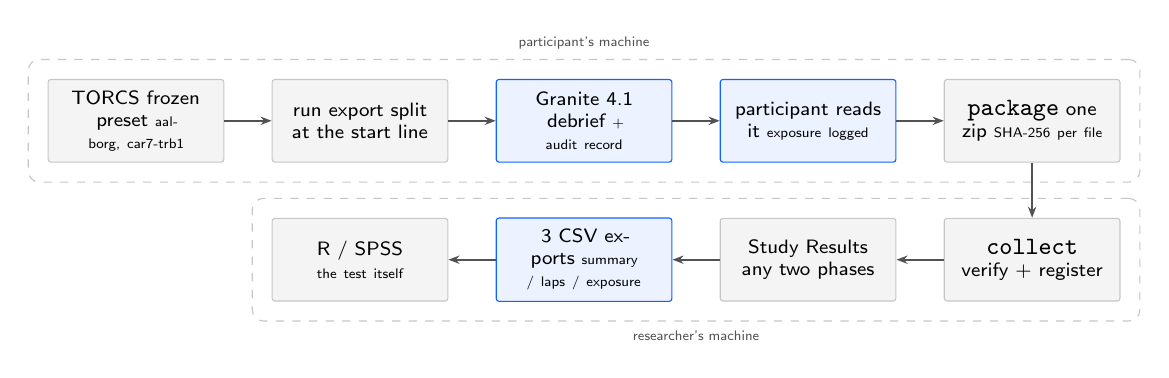
\begin{tikzpicture}[
    font=\scriptsize,
    box/.style={draw=cline,fill=cwash,rounded corners=1pt,inner sep=4pt,
                text width=1.95cm,align=center,minimum height=1.05cm},
    hot/.style={box,draw=cblue,fill=cblue!8},
    ar/.style={-{Stealth[length=4pt]},draw=cgray,thick}]
    \node[box]              (drive)  {TORCS\ frozen preset\ \tiny aalborg, car7-trb1};
    \node[box,right=6mm of drive] (split) {run export\ split at the\ start line};
    \node[hot,right=6mm of split] (coach) {Granite 4.1\ debrief\ \tiny + audit record};
    \node[hot,right=6mm of coach] (read)  {participant\ reads it\ \tiny exposure logged};
    \node[box,right=6mm of read]  (pack)  {\code{package}\ one zip\ \tiny SHA-256 per file};
    \node[box,below=7mm of pack]  (coll)  {\code{collect}\ verify +\ register};
    \node[box,left=6mm of coll]   (study) {Study Results\ any two phases};
    \node[hot,left=6mm of study]  (csv)   {3 CSV exports\ \tiny summary / laps / exposure};
    \node[box,left=6mm of csv]    (stats) {R / SPSS\ \tiny the test itself};
    \draw[ar] (drive) -- (split);
    \draw[ar] (split) -- (coach);
    \draw[ar] (coach) -- (read);
    \draw[ar] (read)  -- (pack);
    \draw[ar] (pack)  -- (coll);
    \draw[ar] (coll)  -- (study);
    \draw[ar] (study) -- (csv);
    \draw[ar] (csv)   -- (stats);
    \begin{scope}[on background layer]
      \node[draw=cline,dashed,rounded corners,fit=(drive)(pack),inner sep=7pt,
            label={[font=\tiny,color=cgray]above:participant's machine}] {};
      \node[draw=cline,dashed,rounded corners,fit=(coll)(stats),inner sep=7pt,
            label={[font=\tiny,color=cgray]below:researcher's machine}] {};
    \end{scope}
  \end{tikzpicture}
  \end{center}
  \vspace{0.2em}
  {\footnotesize
  The participant installs Apex on their own laptop, so everything between the two
  dashed boxes has to survive email or a memory stick. A handover is therefore
  \kw{one file with a digest of every member}: a study that silently analyses eleven
  of a participant's twelve laps has a hole no later check can find.}
\end{frame}

% ==========================================================================
\begin{frame}{Collecting data: the participant never sees a command line}{\code{Collect Data} --- conditions frozen, phase chosen, checks forced}
  \shot{01-collect-control}
  \caphere{The control arm's own capture page. \kw{The setup is not a choice}: track, car,
  lap count and window size are locked to \code{apex-study-v1}, because a different
  rendering size is a different condition. The phase dropdown is the whole allocation
  interface --- \emph{Baseline}, \emph{Coached}, \emph{Control}, \emph{Familiarisation}
  --- and whatever is picked is written into every lap file's header.}
\end{frame}

% ==========================================================================
\begin{frame}{Whose lap is this?}{\code{Garage} --- identity rides inside the file, not in a side table}
  \shotw{02-garage}{1.0}
  \vspace{0.3em}
  {\footnotesize
  Each lap CSV carries \code{\# driver:}, \code{\# phase:} and \code{\# setup:} in its own
  header. Copy it to another machine, pool it with twenty others, open it in a year ---
  it still says who drove it and under what condition. Laps that carry \emph{no} identity
  are \kw{dropped from the study export rather than pooled into an anonymous group}: a lap
  that cannot be attributed cannot stand on either side of a comparison.}
\end{frame}

% ==========================================================================
\begin{frame}{The coaching itself}{\code{Lap Analysis} --- IBM Granite 4.1, running locally, citing its evidence}
  \shot{03-analysis}
  \caphere{Participant B0826, baseline lap 2. The finding on the right is the real model
  output: \emph{``Brake application needs review\dots use one progressive brake application
  and one controlled release''}, with \kw{four evidence citations} underneath it
  (\code{T7 brake applications: 2 count}, \code{T7 coast distance: 135 m}, \dots).
  A finding whose citations do not survive re-validation against the telemetry
  \kw{is not published} --- the model cannot assert a number the lap does not contain.}
\end{frame}

% ==========================================================================
\begin{frame}{Advice at the place it happened}{\code{Review} --- one corner at a time, not a wall of text}
  \begin{columns}[T]
  \begin{column}{0.46\textwidth}
    \shoth{04-review}{0.62}
  \end{column}
  \begin{column}{0.54\textwidth}
    \vspace{0.6em}\footnotesize
    A participant does not need to be told how their lap went --- they drove it. They
    need to know that \emph{at Turn 1} they split the braking, and what to do instead.
    \begin{itemize}\footnotesize
      \item Corners in the order they are driven, with what each one cost.
      \item The track map marks the stretch; the traces beside it zoom to the same
        span, so the claim and the evidence are on screen together.
      \item Beside it (cropped out here) the \kw{race footage of that corner}, cut with
        ffmpeg and driven by the same transport as the marker, so the picture and the
        dot are at the same point on track. Video is shown to the driver only ---
        \kw{it is never sent to the model}.
      \item How long each corner stays open is now recorded (slide~17).
    \end{itemize}
    \vspace{0.3em}
    {\color{cgray}\scriptsize The video pane is cropped because a video surface is composited
    by the graphics stack and cannot be captured from an unmapped window --- it renders
    black in a headless screenshot, which would read as a broken feature.}
  \end{column}
  \end{columns}
\end{frame}

% ==========================================================================
\begin{frame}{The study screen}{\code{Study Results} --- compare any two phases, on real collected data}
  \shot{05-study-coached}
  \caphere{All five collected phases, with each participant's prior-experience
  questionnaire on the same row. Until last week this screen \kw{hard-coded
  baseline vs coached} and could not display a control participant at all ---
  the arm the study depends on was invisible in the tool built to see it.}
\end{frame}

% ==========================================================================
\begin{frame}{The same screen, the other arm}{The pickers are the fix: any design with named phases is now visible}
  \shot{06-study-control}
  \caphere{\code{baseline} against \code{control} for C0826. The headline counts only
  participants who drove \emph{both} of the chosen phases (1 of 3), so the denominator
  cannot quietly include people who only ever drove one. Three-arm designs, repeated
  interventions and a familiarisation phase all work without a code change.}
\end{frame}

% ==========================================================================
\begin{frame}{Provenance: what the model was asked, and answered}{One JSON record per coaching run --- success or failure}
  \begin{columns}[T]
  \begin{column}{0.52\textwidth}
    \shoth{07-audit}{0.66}
  \end{column}
  \begin{column}{0.48\textwidth}
    \vspace{0.4em}\footnotesize
    Every run of every provider leaves a self-contained record: the frozen evidence
    packet, the exact prompt, the raw streamed answer, and what Apex did with it.
    \begin{itemize}\footnotesize
      \item \kw{New this week:} \code{driver}, \code{phase} and \code{setup} are in the
        record. It used to name only the lap \emph{file} --- and a file name is not a
        participant. Files are renamed on import, pooled across machines, and read
        months later by somebody who was not there.
      \item This trail is also \kw{the only record of what each participant was actually
        told}, which is what the adherence measure reads (slide~18).
      \item A stored report is re-shown only if provider, lap, reference, model,
        prompt version \emph{and} evidence packet all still match, and its citations
        pass validation again. Audit files are treated as untrusted input.
    \end{itemize}
  \end{column}
  \end{columns}
\end{frame}

% ==========================================================================
\begin{frame}{What is measured --- and what the software refuses to guess}
  \vspace{-0.2em}
  \begin{center}\footnotesize
  \begin{tabular}{@{}L{3.3cm}L{5.0cm}L{5.6cm}@{}}
    \toprule
    \textbf{Measure} & \textbf{How} & \textbf{Why it is defined that way} \
    \midrule
    Lap time & \code{best}, \code{mean}, \code{sd} per phase &
      \code{sd} is a \emph{population} sd: these laps are the whole phase, not a
      sample of it. It doubles as a consistency outcome. \
    Leaving the track & \emph{episodes}, not sample proportion &
      One 2\,s excursion and ten line-clipping wobbles are different problems; a
      per-sample ratio hides which. \
    Damage & rising edges \emph{within} a lap &
      Damage accumulates over a race, so lap 3's start is lap 2's end. \
    Start-line lap & discarded &
      A standing start would systematically slow every baseline and manufacture an
      improvement. \
    \midrule
    Missing channel & \kw{blank, never 0} &
      Counting an unrecorded signal as ``no excursions'' quietly rewards the
      participants whose data was incomplete. \
    Significance & \kw{not computed} &
      Deliberate, documented, and locked by tests. The software produces rows; the
      test is the analyst's. \
    \bottomrule
  \end{tabular}
  \end{center}
  \vspace{0.2em}
  {\footnotesize\color{cgray} Blank cells must be read as missing (\code{na.strings=""}),
  not as zero. That is the entire point of the distinction.}
\end{frame}

% ==========================================================================
\begin{frame}{What changed since the last meeting}{Six items, all driven by problems the real data exposed}
  \vspace{-0.2em}
  \begin{center}\footnotesize
  \begin{tabular}{@{}L{0.9cm}L{5.6cm}L{7.4cm}@{}}
    \toprule
    & \textbf{Change} & \textbf{What it fixed} \
    \midrule
    6.2 & Control arm in the capture wizard &
      The control participant can be collected through the same guided page ---
      no command line for the facilitator. \
    6.3 & Study screen compares \emph{any} two phases &
      The control arm was previously invisible in the analysis tool. \
    6.1 & Background columns in the GUI export &
      The screen showed a questionnaire the exported file did not carry. \
    6.4 & \code{study-laps}: one row per lap &
      A phase summary has no slope. Learning curves and mixed-effects models
      need every observation. \
    6.5 & \kw{Coaching exposure measured} &
      ``Delivered'' was being read as ``received''. See slide~17. \
    --- & \kw{Advice adherence measured} &
      ``Received'' was being read as ``acted on''. See slide~18. \
    \bottomrule
  \end{tabular}
  \end{center}
  \vspace{0.3em}
  {\footnotesize Plus three defects that only appeared once real handovers existed:
  the documented \code{collect}\,$\rightarrow$\,\code{study-summary} path
  \kw{produced nothing at all}; every export on every machine contained a
  \kw{phantom participant} (the shipped demo carries a real identity); and
  \kw{one header-only export file aborted the import of four participants}.}
\end{frame}

% ==========================================================================
\begin{frame}{The first real data}{Three participants, five phases, fifteen laps --- Aalborg, car7-trb1}
  \vspace{-0.2em}
  \begin{center}\footnotesize
  \begin{tabular}{@{}llR{1.2cm}R{1.2cm}R{1.0cm}R{1.5cm}R{1.5cm}L{2.6cm}@{}}
    \toprule
    \textbf{ID} & \textbf{Phase} & \textbf{Best} & \textbf{Mean} & \textbf{SD} &
    \textbf{Off track} & \textbf{Time off} & \textbf{Prior experience} \
    \midrule
    0823  & baseline & 112.30 & 119.50 & 5.46 & 76 & 123.04\,s & games a few times \
    \midrule
    B0826 & baseline & 119.62 & 124.77 & 3.70 & 74 & 120.97\,s & games a few times \
    B0826 & \textbf{coached}  & 126.12 & \textbf{132.16} & 5.03 & 82 & 178.82\,s & \
    \midrule
    C0826 & baseline & 105.98 & 116.38 & 8.05 & 71 & 123.58\,s & games weekly \
    C0826 & \textbf{control}  & 114.19 & \textbf{118.08} & 3.17 & 64 & \phantom{0}94.71\,s & \
    \bottomrule
  \end{tabular}
  \end{center}
  \vspace{0.4em}
  \begin{columns}[T]
  \begin{column}{0.54\textwidth}\footnotesize
  \textbf{On the face of it, both got slower.}\
  Coached arm $+7.4$\,s on the mean; control arm $+1.7$\,s.
  \kw{With one participant per arm this means nothing} --- it is reported
  because it is what the instrument produced, not because it is a result.
  \end{column}
  \begin{column}{0.46\textwidth}\footnotesize
  \textbf{The off-track numbers are real.}\
  74--82 excursions per phase looked like a bug. Checked against the raw channel:
  \code{|track\_pos| > 1} for \kw{20.5\%} of samples, reaching $\pm2.6$. Aalborg is
  narrow and these are novices. Good news for the safety metric's dynamic range.
  \end{column}
  \end{columns}
\end{frame}

% ==========================================================================
\begin{frame}{Why the summary row points the wrong way}{The per-lap export exists for exactly this}
  \vspace{-0.1em}
  \begin{center}\footnotesize
  \begin{tabular}{@{}llR{1.7cm}R{1.7cm}R{1.7cm}L{4.3cm}@{}}
    \toprule
    \textbf{ID} & \textbf{Phase} & \textbf{Lap 1} & \textbf{Lap 2} & \textbf{Lap 3} & \
    \midrule
    B0826 & baseline & \textbf{119.62} & 128.14 & 126.56 & fastest lap is the \emph{first} \
    B0826 & coached  & 138.44 & 131.92 & \textbf{126.12} & \good{$-12.3$\,s across three laps} \
    \midrule
    C0826 & baseline & 125.60 & \textbf{105.98} & 117.56 & \
    C0826 & control  & 114.19 & 121.95 & 118.10 & no trend \
    \bottomrule
  \end{tabular}
  \end{center}
  \vspace{0.5em}
  \begin{itemize}\footnotesize
    \item B0826's coached phase holds \kw{the steepest descent in the whole dataset}
      --- and their baseline phase got \emph{worse} after lap 1.
    \item So the phase mean, which says ``$7.4$\,s slower'', is largely the first
      coached lap. \kw{A single number per phase has no slope}, and the direction it
      reports here is arguably the opposite of what the laps show.
    \item This is the argument for \code{study-laps} (one row per lap) and for a
      mixed-effects model with laps nested in participants: it uses all 15
      observations and lets practice be \emph{estimated} rather than assumed away.
    \item It is also the argument for \kw{more than three laps per phase} --- the
      curve is still falling when the phase ends.
  \end{itemize}
\end{frame}

% ==========================================================================
\begin{frame}{Dose: did they actually read it?}{New --- and the reason it matters most at this sample size}
  \begin{columns}[T]
  \begin{column}{0.53\textwidth}\footnotesize
  With one participant per arm the \emph{between-arm} comparison is underpowered by
  construction. The one causal argument that does \kw{not} depend on the arms being
  alike is \kw{dose and response}: within the coached arm, did the people who
  engaged more improve more?

  \vspace{0.4em}
  That needs the dose to be a measurement. Previously nothing was recorded ---
  ``a report was generated'' was standing in for ``a participant read it''.

  \vspace{0.5em}
  Two kinds of view are timed, deliberately kept apart:
  \begin{itemize}\footnotesize
    \item \code{corner} --- the review window open on one corner
    \item \code{report} --- the findings panel on the analysis screen
  \end{itemize}
  Somebody who read the panel and never opened a single corner is a real case, and
  pooling the two would hide them. The two clocks never overlap, so they can be added.
  \end{column}
  \begin{column}{0.47\textwidth}
  \vspace{0.2em}\footnotesize
  \textbf{Five columns, per participant per phase}
  \begin{center}\scriptsize
  \begin{tabular}{@{}L{3.4cm}L{3.3cm}@{}}
    \toprule
    \code{review\_seconds} & corner review time \
    \code{review\_corners} & how many views \
    \code{review\_corners\_seen} & how many \emph{distinct} \
    \code{advice\_seconds} & with an instruction on screen \
    \code{report\_seconds} & findings panel \
    \bottomrule
  \end{tabular}
  \end{center}
  \vspace{0.3em}
  \textbf{Three rules that make it honest}
  \begin{itemize}\scriptsize
    \item The dose belongs to the phase \emph{being read}, not the one driven next.
      Reading the second run's laps afterwards cannot have caused it.
    \item \kw{No log = blank; empty log = 0.} ``Nobody recorded it'' and ``they read
      nothing'' are different facts, and only one can be fixed.
    \item Views under 1\,s are not counted --- arrowing through a list is keystrokes,
      not attention.
  \end{itemize}
  \end{column}
  \end{columns}
\end{frame}

% ==========================================================================
\begin{frame}{Adherence: did they then do it?}{The missing middle term between advice and lap time}
  \begin{columns}[T]
  \begin{column}{0.52\textwidth}\footnotesize
  Advice that does not work and advice nobody acted on \kw{produce the same lap times}.
  Without this term a null result cannot be read at all.

  \vspace{0.4em}
  For every instruction the debrief actually gave --- taken from the audit trail, so
  it is what was really said --- the same measurement is taken in the baseline run and
  in the second run, and the shift is expressed in \kw{baseline standard deviations}.

  \vspace{0.5em}
  Three things make the comparison defensible:
  \begin{itemize}\scriptsize
    \item \textbf{One anchor lap.} Corner numbering comes from apex detection; detect
      twice on two laps and one extra dip renames everything after it. Every lap of
      both runs is measured on \emph{one} anchor's grid.
    \item \textbf{Absolute measurements, not gaps.} A gap is measured against a
      reference that differs between runs.
    \item \textbf{Across runs only.} Nothing is shown to the participant between one
      lap and the next, so a lap-2-to-lap-3 change is familiarity, not compliance.
    \end{itemize}
  \end{column}
  \begin{column}{0.48\textwidth}
  \vspace{0.3em}
  \begin{center}\footnotesize
  \begin{tabular}{@{}lR{1.3cm}R{1.3cm}R{1.5cm}@{}}
    \toprule
    & \textbf{advised} & \textbf{followed} & \textbf{shift (sd)} \
    \midrule
    B0826 coached & 4 & 1 & \good{$+0.67$} \
    C0826 control & 4 & 0 & \bad{$-0.65$} \
    \bottomrule
  \end{tabular}
  \end{center}
  \vspace{0.5em}
  {\footnotesize
  The control participant is scored against \emph{the debrief written for their own
  baseline} --- generated, never shown to them. That is the right comparator: it asks
  whether the coached participant moved toward the advice more than someone who
  never saw it.

  \vspace{0.4em}
  \kw{n = 1 in each row.} The shape of the evidence is what matters here, not the
  numbers: this is the column a dose--response argument is finally able to use.}
  \end{column}
  \end{columns}
\end{frame}

% ==========================================================================
\begin{frame}{How the instrument is kept honest}{Because a measurement tool that is wrong is worse than none}
  \begin{columns}[T]
  \begin{column}{0.48\textwidth}\footnotesize
  \textbf{Discipline}
  \begin{itemize}\footnotesize
    \item \kw{737 tests}, 17 skipped; linting clean. Every behavioural change here
      was \kw{proved failing before it was made to pass} --- not asserted to have been.
    \item Telemetry truth lives in one Qt-free core; the GUI and CLI render it and
      never recompute it, so the two cannot drift.
    \item Handovers verify a SHA-256 per member; a mismatch stops the whole unpack,
      because half a participant's session is worse than none --- it looks complete.
  \end{itemize}
  \end{column}
  \begin{column}{0.52\textwidth}\footnotesize
  \textbf{Two things caught this week by \emph{running} it, not reading it}
  \begin{itemize}\footnotesize
    \item Driving the frozen build end to end: 3 views written, \kw{2 arrived}.
      Cause --- files that cross machines were read as plain UTF-8, so a
      byte-order mark silently ate the first line. For a manifest that means an
      entire handover imports as \kw{nobody's laps}, with no error.
    \item Looking at the real workspace: 16 exposure views recorded against two
      participants that were actually \kw{the researcher clicking through their
      laps} on the analysis machine. A session collected from a handover was driven
      somewhere else, so it can never be a dose. Fixed, and the false rows
      quarantined.
  \end{itemize}
  \vspace{0.2em}
  {\color{cgray}\scriptsize Both are the same lesson as the broken
  \code{collect}\,$\rightarrow$\,\code{study-summary} path: defects in a study
  instrument show up when it is run against real data, not when it is reviewed.}
  \end{column}
  \end{columns}
\end{frame}

% ==========================================================================
\begin{frame}{Threats to validity --- stated, not hidden}
  \vspace{-0.2em}
  \begin{center}\footnotesize
  \begin{tabular}{@{}L{4.2cm}L{5.1cm}L{4.6cm}@{}}
    \toprule
    \textbf{Threat} & \textbf{Status} & \textbf{Mitigation / decision needed} \
    \midrule
    \kw{Practice confound} & Addressed in design & Control arm implemented and
      collected; needs \emph{n}. \
    \kw{Sample size} & \bad{n = 1 per arm} & Recruitment plan --- the ask of this
      meeting. \
    \kw{Laps per phase} & 3; curve still falling at lap 3 & Raise to 5? Cheaper than
      any code change and must be decided \emph{before} the next participant. \
    \kw{\code{best\_lap\_s} is biased} & Minimum of 3 draws; falls as \emph{n} rises &
      Report \code{mean\_lap\_s} as primary, \code{best} as secondary. \
    \kw{Allocation} & Manual list, no audit trail & Item 6.6: generate and lock
      participant\,$\rightarrow$\,condition in Apex. \
    \kw{No pre-registration} & None yet & Primary outcome, stopping rule and
      power analysis before the next participant. \
    \kw{Exposure only from now} & Earlier handovers carry none & Their dose columns
      export \emph{blank}, which is correct --- not zero. \
    \bottomrule
  \end{tabular}
  \end{center}
\end{frame}

% ==========================================================================
\begin{frame}{Next steps, and what I need from you}
  \begin{columns}[T]
  \begin{column}{0.52\textwidth}
  \textbf{\normalsize Software --- roughly one week}
  \begin{itemize}\footnotesize
    \item \kw{6.6 Randomised allocation.} Generate and lock the
      participant\,$\rightarrow$\,condition mapping inside Apex, with a record of
      when it was drawn. Currently a manual list: easy to get wrong, and nothing
      proves it was not.
    \item Raise the preset to \kw{5 laps per phase} once the current test round
      is finished (deferred deliberately: it would add two laps to every test run).
    \item Surface exposure and adherence on the Study screen, not only in the CSVs.
  \end{itemize}
  \vspace{0.4em}
  \textbf{\normalsize Study}
  \begin{itemize}\footnotesize
    \item Recruit. Everything else is now waiting on participants.
    \item Pre-register primary outcome + analysis before the next one drives.
  \end{itemize}
  \end{column}
  \begin{column}{0.48\textwidth}
  \textbf{\normalsize Decisions I need}
  \begin{enumerate}\footnotesize
    \item[\textbf{1.}] \kw{How many participants can we realistically recruit, and by
      when?} The design is 2 arms; anything under roughly 12--16 per arm makes the
      between-arm test decorative, and the dose--response argument becomes the
      primary one.
    \item[\textbf{2.}] \kw{3 laps or 5?} Slide 15 says the coached phase was still
      improving at lap 3.
    \item[\textbf{3.}] \kw{Ethics / data handling.} One participant's screen
      recording was committed and pushed to a GitHub repository before the
      \code{.gitignore} rule existed. Options: accept, remove from the working tree,
      or rewrite history and force-push. \textbf{Your call} --- I have not touched it.
    \item[\textbf{4.}] Is a familiarisation phase (not counted) worth the extra
      participant time?
  \end{enumerate}
  \end{column}
  \end{columns}
\end{frame}

% ==========================================================================
\begin{frame}{Notes on this deck}{So nothing here has to be taken on trust}
  \begin{itemize}\footnotesize
    \item Every screenshot is the \kw{real application}, rendered by driving it
      programmatically against a copy of the study workspace
      (\code{docs/slides/make-progress-screenshots.py}). No mock-ups.
    \item The coaching content is \kw{IBM Granite 4.1 (3B, Q4\_K\_M) running locally},
      restored from the audit record it wrote at the time --- not regenerated for
      the deck and not a deterministic stand-in.
    \item Participant identifiers are pseudonymous; they are what the study records.
      No names, and free text is not collected anywhere.
    \item The two figures that are cropped are marked as such, and why.
    \item Numbers on slides 14--15 and 18 come from
      \code{racecoach study-summary}, \code{study-laps} and \code{study-adherence}
      run against the real workspace on 27 August 2026.
  \end{itemize}
  \vspace{0.8em}
  \begin{center}
  {\color{cblue}\rule{0.4\textwidth}{1.1pt}}\par\vspace{0.6em}
  {\footnotesize\color{cgray}Detail behind every claim:
  \code{docs/STUDY\_CAN\_WE\_SHOW\_IMPROVEMENT.md}}
  \end{center}
\end{frame}

\end{document}
